\documentclass{article}

\usepackage{tikz} 
\usetikzlibrary{automata, positioning, arrows} 

\usepackage{amsthm}
\usepackage{amsfonts}
\usepackage{amsmath}
\usepackage{amssymb}
\usepackage{fullpage}
\usepackage{color}
\usepackage{parskip}
\usepackage{hyperref}
  \hypersetup{
    colorlinks = true,
    urlcolor = blue,       % color of external links using \href
    linkcolor= blue,       % color of internal links 
    citecolor= blue,       % color of links to bibliography
    filecolor= blue,        % color of file links
    }
    
\usepackage{listings}
\usepackage[utf8]{inputenc}                                                    
\usepackage[T1]{fontenc}                                                       

\definecolor{dkgreen}{rgb}{0,0.6,0}
\definecolor{gray}{rgb}{0.5,0.5,0.5}
\definecolor{mauve}{rgb}{0.58,0,0.82}

\lstset{frame=tb,
  language=haskell,
  aboveskip=3mm,
  belowskip=3mm,
  showstringspaces=false,
  columns=flexible,
  basicstyle={\small\ttfamily},
  numbers=none,
  numberstyle=\tiny\color{gray},
  keywordstyle=\color{blue},
  commentstyle=\color{dkgreen},
  stringstyle=\color{mauve},
  breaklines=true,
  breakatwhitespace=true,
  tabsize=3
}

\newtheoremstyle{theorem}
  {\topsep}   % ABOVESPACE
  {\topsep}   % BELOWSPACE
  {\itshape\/}  % BODYFONT
  {0pt}       % INDENT (empty value is the same as 0pt)
  {\bfseries} % HEADFONT
  {.}         % HEADPUNCT
  {5pt plus 1pt minus 1pt} % HEADSPACE
  {}          % CUSTOM-HEAD-SPEC
\theoremstyle{theorem} 
   \newtheorem{theorem}{Theorem}[section]
   \newtheorem{corollary}[theorem]{Corollary}
   \newtheorem{lemma}[theorem]{Lemma}
   \newtheorem{proposition}[theorem]{Proposition}
\theoremstyle{definition}
   \newtheorem{definition}[theorem]{Definition}
   \newtheorem{example}[theorem]{Example}
\theoremstyle{remark}    
  \newtheorem{remark}[theorem]{Remark}

\title{CPSC-406 Report}
\author{Nathan Carnnahan  \\ Chapman University}

\date{\today} 

\begin{document}

\maketitle

\begin{abstract}
\end{abstract}

\setcounter{tocdepth}{3}
\tableofcontents
\clearpage
\section{Introduction}

\section{Introduction}\label{intro}

\section{Week by Week}\label{homework}

\subsection{Week 1}
\subsubsection*{HW1 -- DFA Exercises}

\paragraph{Exercise 1}

We are given two DFAs $A_1$ and $A_2$.

\subparagraph{Accepted Words Table}

\begin{center}
\begin{tabular}{c|c|c}
$w$ & Accepted by $A_1$? & Accepted by $A_2$? \\ \hline
$aaa$ & No & Yes \\
$aab$ & Yes & No \\
$aba$ & No & No \\
$abb$ & No & No \\
$baa$ & No & Yes \\
$bab$ & No & No \\
$bba$ & No & No \\
$bbb$ & No & No \\
\end{tabular}
\end{center}

\subparagraph{Language Descriptions}

\begin{itemize}
\item $L(A_1)$: all strings over $\{a,b\}$ that start with $a$ and end with an odd number of $b$'s.
\item $L(A_2)$: all strings over $\{a,b\}$ that end with at least two consecutive $a$'s.
\end{itemize}

\vspace{1em}

\paragraph{Exercise 2 -- Designing DFAs}

\subparagraph{1. Words that end with $ab$}

\begin{center}
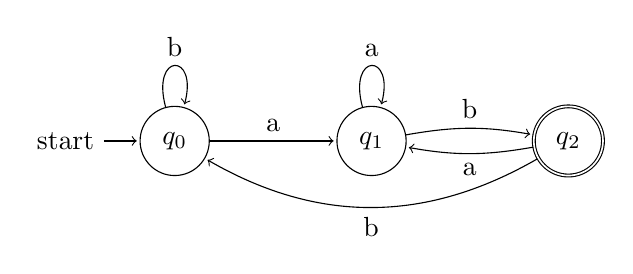
\begin{tikzpicture}[shorten >=1pt,node distance=2.5cm,on grid,auto]
\node[state,initial] (q0) {$q_0$};
\node[state] (q1) [right=of q0] {$q_1$};
\node[state,accepting] (q2) [right=of q1] {$q_2$};

\path[->]
(q0) edge [loop above] node {b} ()
     edge node {a} (q1)
(q1) edge [loop above] node {a} ()
     edge [bend left = 10] node {b} (q2)
(q2) edge [bend left = 10] node {a} (q1)
     edge[bend left=30] node {b} (q0);
\end{tikzpicture}
\end{center}

\subparagraph{2. Words that contain $aba$}

\begin{center}
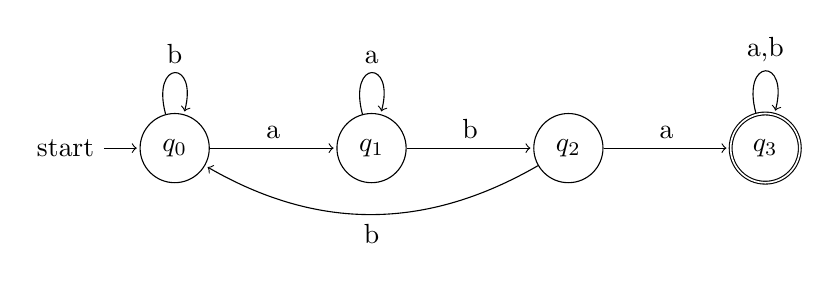
\begin{tikzpicture}[shorten >=1pt,node distance=2.5cm,on grid,auto]
\node[state,initial] (q0) {$q_0$};
\node[state] (q1) [right=of q0] {$q_1$};
\node[state] (q2) [right=of q1] {$q_2$};
\node[state,accepting] (q3) [right=of q2] {$q_3$};

\path[->]
(q0) edge [loop above] node {b} ()
     edge node {a} (q1)
(q1) edge [loop above] node {a} ()
     edge node {b} (q2)
(q2) edge node {a} (q3)
     edge[bend left] node {b} (q0)
(q3) edge [loop above] node {a,b} ();
\end{tikzpicture}
\end{center}

\subparagraph{3. Odd number of $a$'s and odd number of $b$'s}

States represent parity: $(a\text{-parity}, b\text{-parity})$.

\begin{center}
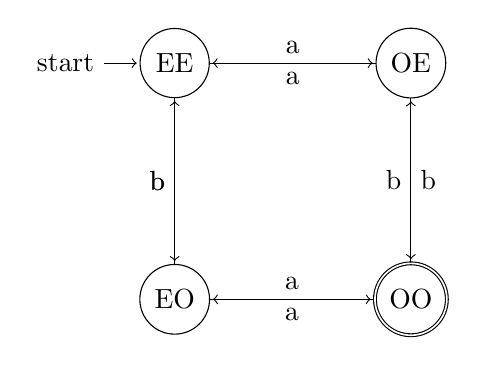
\begin{tikzpicture}[shorten >=1pt,node distance=3cm,on grid,auto]
\node[state,initial] (EE) {EE};
\node[state] (OE) [right=of EE] {OE};
\node[state] (EO) [below=of EE] {EO};
\node[state,accepting] (OO) [right=of EO] {OO};

\path[->]
(EE) edge node {a} (OE)
     edge node[left] {b} (EO)
(OE) edge node {a} (EE)
     edge node {b} (OO)
(EO) edge node {a} (OO)
     edge node {b} (EE)
(OO) edge node {a} (EO)
     edge node {b} (OE);
\end{tikzpicture}
\end{center}

\subparagraph{4. Even number of $a$'s and odd number of $b$'s}

Same automaton as above, but accepting state is EO.

\subparagraph{5. Any three consecutive characters contain at least one $a$}

Equivalent to forbidding substring $bbb$.

\begin{center}
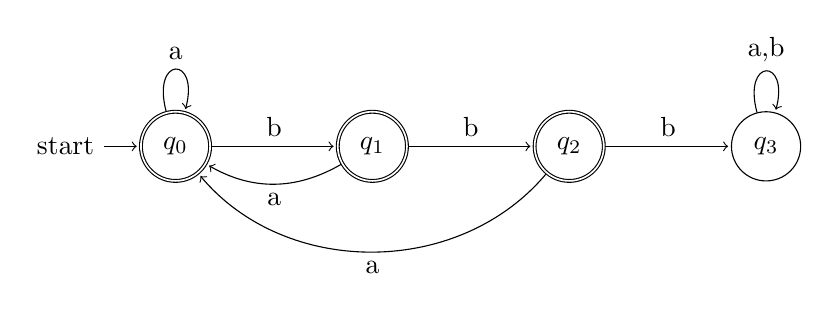
\begin{tikzpicture}[shorten >=1pt,node distance=2.5cm,on grid,auto]
\node[state,initial,accepting] (q0) {$q_0$};
\node[state,accepting] (q1) [right=of q0] {$q_1$};
\node[state,accepting] (q2) [right=of q1] {$q_2$};
\node[state] (q3) [right=of q2] {$q_3$};

\path[->]
(q0) edge node {b} (q1)
     edge[loop above] node {a} ()
(q1) edge node {b} (q2)
     edge[bend left] node {a} (q0)
(q2) edge node {b} (q3)
     edge[bend left = 50] node {a} (q0)
(q3) edge[loop above] node {a,b} ();
\end{tikzpicture}
\end{center}

\subparagraph{6. Words that contain $bbb$}

\begin{center}
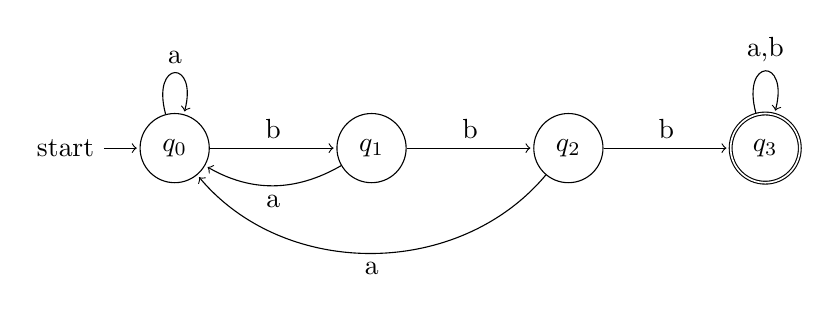
\begin{tikzpicture}[shorten >=1pt,node distance=2.5cm,on grid,auto]
\node[state,initial] (q0) {$q_0$};
\node[state] (q1) [right=of q0] {$q_1$};
\node[state] (q2) [right=of q1] {$q_2$};
\node[state,accepting] (q3) [right=of q2] {$q_3$};

\path[->]
(q0) edge node {b} (q1)
     edge[loop above] node {a} ()
(q1) edge node {b} (q2)
     edge[bend left] node {a} (q0)
(q2) edge node {b} (q3)
     edge[bend left = 50] node {a} (q0)
(q3) edge[loop above] node {a,b} ();
\end{tikzpicture}
\end{center}

\paragraph{Observation}

\begin{itemize}
\item Problems 3 and 4 use the same parity structure; only the accepting state changes.
\item Problems 5 and 6 use the same “count consecutive $b$'s” structure; one treats reaching three $b$'s as rejection, the other as acceptance.
\item Problems 1 and 2 track progress toward matching a pattern.
\end{itemize}

\subsection{Week 2}
\subsubsection*{HW2 -- Operations on automata}

\paragraph{Exercise 1 (Product automata).}

Throughout, $\Sigma=\{a,b\}$.

\medskip
\textbf{1. Description of $L(A^{(1)})$ and $L(A^{(2)})$.}

\medskip
\underline{$A^{(1)}$:}

The accepting states are $\{2,4\}$ and state $3$ is a non-accepting sink (it loops on both $a$ and $b$).
From state $2$, reading $a$ goes to the sink; from state $4$, reading $b$ goes to the sink.
Thus, once the first symbol is read, the letters must alternate in order to avoid the sink.

Therefore,
\[
L(A^{(1)})=\{\,w\in\{a,b\}^* : |w|\ge 1 \text{ and $w$ contains no substring $aa$ or $bb$}\,\}.
\]

Equivalently,
\[
L(A^{(1)}) = a(ba)^*(\varepsilon \mid b)\ \cup\ b(ab)^*(\varepsilon \mid a).
\]

\medskip
\underline{$A^{(2)}$:}

The only accepting state is $2$. From state $1$, reading $b$ leads to a sink.
Reading $a$ moves $1 \to 2$, and from $2$ any symbol returns to $1$.

Thus a word must:
\begin{itemize}
\item start with $a$,
\item have odd length,
\item have $a$ in every odd position.
\end{itemize}

Hence,
\[
L(A^{(2)}) = a\big((a\mid b)a\big)^*.
\]

\medskip
\textbf{2. Intersection automaton $A = A^{(1)} \times A^{(2)}$.}

\begin{itemize}
\item States: $Q = Q_1 \times Q_2$
\item Start state: $(1,1)$
\item Accepting states:
\[
F = F_1 \times F_2 = \{2,4\}\times\{2\}
\]
\item Transition function:
\[
\delta((p,q),x) = (\delta_1(p,x), \delta_2(q,x))
\]
\end{itemize}

The reachable accepting state is $(2,2)$.

\medskip
\textbf{3. Proof that $L(A)=L(A^{(1)})\cap L(A^{(2)})$.}

For any word $w$, by induction on prefixes, after reading $w$ the product automaton is in state
\[
(\delta_1(1,w),\delta_2(1,w)).
\]
Thus $A$ accepts $w$ iff both component automata accept $w$.
Therefore,
\[
L(A)=L(A^{(1)})\cap L(A^{(2)}).
\]

\medskip
\textbf{4. Construction of union automaton $A'$.}

Keep the same product states and transitions, but define the accepting set as
\[
F' = (F_1\times Q_2)\ \cup\ (Q_1\times F_2).
\]
Then $A'$ accepts whenever at least one component accepts, so
\[
L(A') = L(A^{(1)}) \cup L(A^{(2)}).
\]

\bigskip
\paragraph{Exercise 2 (More automata).}

\medskip
\textbf{1. Description of $L(B^{(1)})$ and $L(B^{(2)})$.}

\medskip
\underline{$B^{(1)}$:}

State $p_0$ is accepting. Reading $a$ cycles
\[
p_0 \to p_1 \to p_2 \to p_0,
\]
while $b$ loops at each state.

Thus $B^{(1)}$ accepts exactly when the number of $a$'s is divisible by $3$:
\[
L(B^{(1)})=\{\,w\in\{a,b\}^* : \#_a(w)\equiv 0 \pmod 3\,\}.
\]

\medskip
\underline{$B^{(2)}$:}

State $q_0$ is accepting. The automaton goes to a sink $q_2$ if the substring $aa$ occurs.
Also, $q_1$ is non-accepting, so a word ending in $a$ is rejected.

Hence
\[
L(B^{(2)})=\{\,w\in\{a,b\}^* : \text{$w$ has no substring $aa$ and does not end with $a$}\,\}.
\]
Equivalently,
\[
L(B^{(2)}) = (b \mid ab)^*.
\]

\medskip
\textbf{2. Intersection automaton $B = B^{(1)} \times B^{(2)}$.}

\begin{itemize}
\item Start state: $(p_0,q_0)$
\item Accepting states:
\[
F = \{(p_0,q_0)\}
\]
\item Transition function:
\[
\delta((p_i,q_j),x)=(\delta_1(p_i,x),\delta_2(q_j,x))
\]
\end{itemize}

\medskip
\textbf{3. Proof that $L(B)=L(B^{(1)})\cap L(B^{(2)})$.}

After reading any word $w$, the product automaton is in state
\[
(\delta_1(p_0,w),\delta_2(q_0,w)).
\]
Thus $B$ accepts $w$ iff both component automata accept $w$.
Therefore,
\[
L(B)=L(B^{(1)})\cap L(B^{(2)}).
\]

\medskip
\textbf{4. Construction of union automaton $B'$.}

Using De Morgan's law:
\[
L(B^{(1)})\cup L(B^{(2)})
=
\overline{\ \overline{L(B^{(1)})}\ \cap\ \overline{L(B^{(2)})}\ }.
\]

\begin{enumerate}
\item Complement $B^{(1)}$ and $B^{(2)}$ by swapping accepting and non-accepting states.
\item Construct their product automaton for intersection.
\item Complement the resulting automaton.
\end{enumerate}

This yields $B'$ such that
\[
L(B') = L(B^{(1)}) \cup L(B^{(2)}).
\]


\section{Synthesis}

\section{Evidence of Participation}

\section{Conclusion}\label{conclusion}

\begin{thebibliography}{99}
\bibitem[BLA]{bla} Nathan Carnnahan, \href{https://en.wikipedia.org/wiki/LaTeX}{CPSC-406 Report}, Nathan Carnnahan, 2026.
\end{thebibliography}

\end{document}
